\chapter[MISE EN ŒUVRE]{MISE EN ŒUVRE}
    \section[Introduction partielle]{Introduction partielle}
    Ce chapitre décrira les différentes étapes par lesquelles nous
    sommes passé afin de réaliser notre application web. En premier
    lieu, notre chapitre débutera par l’environnement de réalisation
    de la solution. Ensuite, nous montrerons notre base de données qui a
    comme fondement le diagramme de modèle de domaine vu dans
    le chapitre précèdent. Enfin, nous démontrerons la manière dont
    nous avons choisi notre méthode, construit notre ..............
    \section[Environnement logiciel]{Environnement logiciel}
        \subsection[Choix des langages de développement]{Choix des langages de développement}
            \begin{itemize}
                \setlength{\itemsep}{0pt}
                \item [\ding{226}] \textbf{HTML :} c’est un langage de balisage qui permet de créer et représenter le
                contenu d’une page web et sa structure. Nous l’avons choisi pour organiser nos
                différentes pages web.
                \item [\ding{226}] \textbf{CSS :} c’est un langage de balisage utilisé pour mettre en forme le contenu d’une
                page web. Nous l’avons choisi pour donner une forme agréable aux pages web
                de notre application
                \item [\ding{226}] \textbf{Javascript :} c’est un langage de programmation des scripts utilisé dans les pages
                web interactives. Nous l’avons choisi, car il permet de rendre le contenu mis à
                jour de façon dynamique.
                \item [\ding{226}] \textbf{Python :} est un langage portable, dynamique, extensible, gratuit, qui permet (sans l’imposer) une approche
                modulaire et orienté objet de la programmation. Python est développé depuis 1989 par Guido van Rossum
                et de nombreux contributeurs bénévoles. \cite*{Swinnen2012}
            \end{itemize}
        \subsection[Choix des frameworks]{Choix des frameworks}
            \begin{itemize}
                \setlength{\itemsep}{0pt}
                \item [\ding{226}] \textbf{Bootstrap :}
                \item [\ding{226}] \textbf{Django :} est construit sur une approche très modulaire ; il implémente avec efficacité
                les notions de découplage et de réutilisabilité.
            \end{itemize}
        \subsection[Choix des outils de développement]{Choix des outils de développement}
            \begin{itemize}
                \setlength{\itemsep}{0pt}
                \item [\ding{226}] \textbf{GitHub Desktop :}
                \item [\ding{226}] \textbf{Visual Studio Code :} est un éditeur de code
                extensible développé par Microsoft. Il est un éditeur de code multiplateforme, open source et gratuit,
                supportant une multitude de langages de programmation. \cite*{Wikivsc} Cet outil a était choisi
                pour nous permettre de développer notre application web, mais aussi de rédiger ce document grâce à
                ses nombreuses extensions.
                \item [\ding{226}] \textbf{Microsoft Power BI Desktop :} est l’outil de Microsoft spécifiquement destiné à la visualisation de
                données, à la création de rapports, à l’aide au pilotage de l’entreprise, mais aussi à la
                diffusion de l’information sur différents supports ou plateformes. \cite*{Meyer2021}
            \end{itemize}
        \subsection[Choix du SGBD]{Choix du SGBD}
            \begin{itemize}
                \setlength{\itemsep}{0pt}
                \item [\ding{226}] \textbf{Microsoft SQL Server 2019 :}
            \end{itemize}
    \section[Environnement matériel]{Environnement matériel}
    L'ensemble du travail a était réalisé sur un ordinateur portable
    ayant les caractéristiques suivantes :
    \begin{itemize}
        \setlength{\itemsep}{0pt}
        \item [\ding{228}] \textbf{Fabricant :} Lenovo
        \item [\ding{228}] \textbf{Modèle :} G560
        \item [\ding{228}] \textbf{Type :} x64 (64 bits)
        \item [\ding{228}] \textbf{Processeur :} Intel(R) Core(TM) i5 CPU M 430 2.27 GHz, 2267 MHz, 2 cœurs, 4 processeurs logiques
        \item [\ding{228}] \textbf{Carte graphique :} NVIDIA GeForce 310M, 512 Mo
        \item [\ding{228}] \textbf{Mémoire physique (RAM) installée :} 8,00 Go
        \item [\ding{228}] \textbf{Mémoire physique (HDD) installée :} 298,09 Go
        \item [\ding{228}] \textbf{Système d'exploitation :} Windows 10 Professionnel 22H2
    \end{itemize}
    \section[Présentation de l’interface de l’application]{Présentation de l’interface de l’application}
            \subsection[Interface d’authentification]{Interface d’authentification}
            \begin{figure}[H]
                \centering
                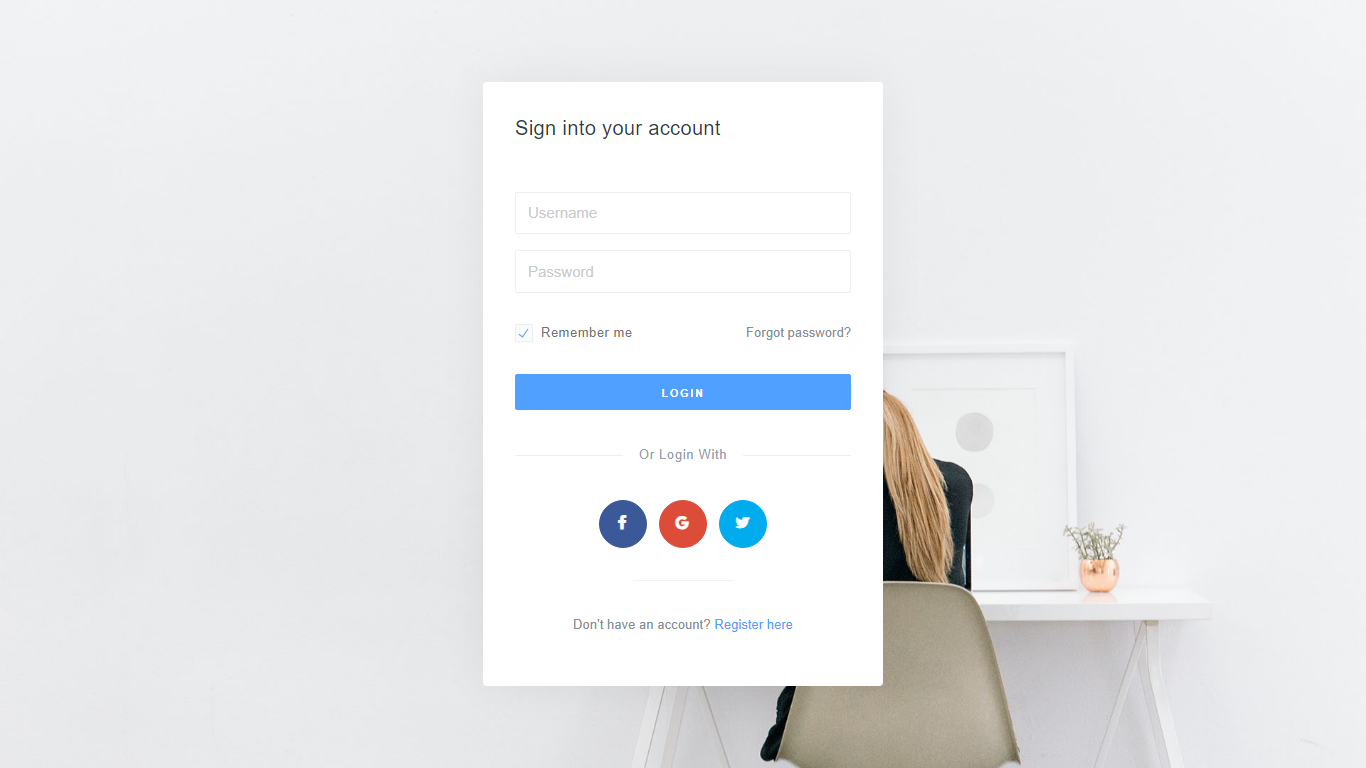
\includegraphics[width=130mm]{images/presentation-de-la-solution/authentifier.png}
                \captionof{figure}{Interface d’authentification}
                \label{fig:mdSysteme}
            \end{figure}
            \subsection[Interface de création de compte client]{Interface de création de compte client}
            \begin{figure}[H]
                \centering
                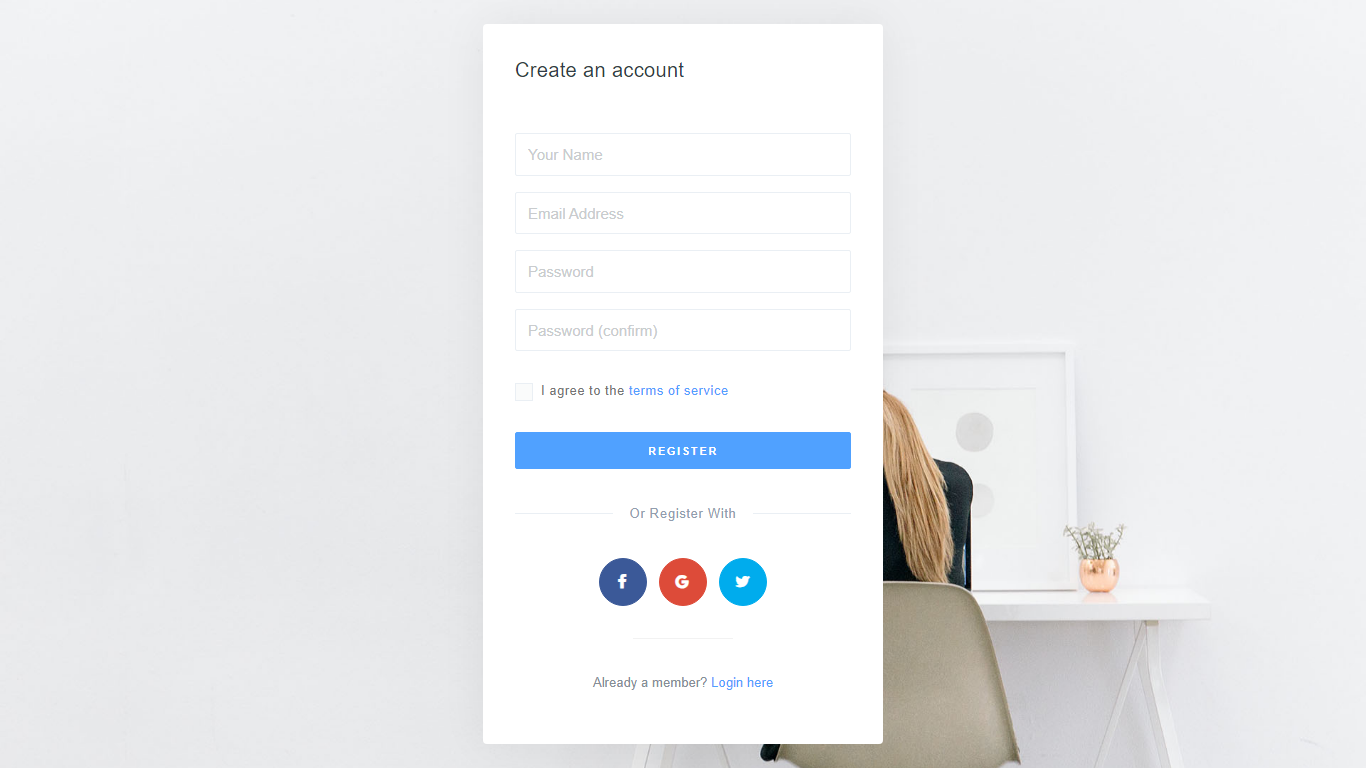
\includegraphics[width=130mm]{images/presentation-de-la-solution/creer-compte.png}
                \captionof{figure}{Interface de création de compte client}
                \label{fig:mdSysteme}
            \end{figure}
    \section[Conclusion partielle]{Conclusion partielle}
    Ce chapitre a était dédié à l’implémentation du système, où nous avons exposé
    les technologies et les outils tout au long du processus de mise en œuvre,
    en plus de détailler l’environnement matériel et les modules de l’application,
    nous avons aussi présenté l’architecture logicielle utilisée. Enfin, nous concluons ce chapitre en présentant l’application à travers quelques
    captures d’écran.
    \par
    Nous voilà arrivés pratiquement à la fin de notre travail ; il est indispensable de récapituler
    de manière condensée le contenu du présent travail de fin d’étude. Le prochain point
    conclu le travail dans sa généralité.